\documentclass[12pt]{article}
\usepackage[UTF8]{ctex}
\usepackage{amsmath,amssymb,amsthm}
\usepackage{graphicx}
\usepackage{subfigure}
\usepackage{booktabs}
\usepackage{multirow}
\usepackage{multicol}
\usepackage{geometry}
\usepackage{listings}
\usepackage{xcolor}
\usepackage{hyperref}

\geometry{a4paper,left=2.5cm,right=2.5cm,top=2.5cm,bottom=2.5cm}

% 代码样式设置
\lstset{
    language=Python,
    basicstyle=\ttfamily\small,
    keywordstyle=\color{blue},
    commentstyle=\color{gray},
    stringstyle=\color{red},
    numbers=left,
    numberstyle=\tiny\color{gray},
    stepnumber=1,
    numbersep=5pt,
    backgroundcolor=\color{white},
    showspaces=false,
    showstringspaces=false,
    showtabs=false,
    frame=single,
    tabsize=4,
    captionpos=b,
    breaklines=true,
    breakatwhitespace=false,
    escapeinside={\%*}{*)}
}

\title{实验三:参数估计与非参数估计}
\author{姓名:\underline{\hspace{3cm}} \quad 学号:\underline{\hspace{3cm}} \quad 专业:\underline{\hspace{3cm}}}
\date{实验日期:}

\begin{document}

\maketitle

\section{实验目的}
\begin{enumerate}
    \item 掌握参数估计方法在模式分类中的应用
    \item 理解非参数估计的基本原理和实现方法
    \item 比较参数方法和非参数方法在不同数据分布下的性能
    \item 分析先验概率对分类器性能的影响
\end{enumerate}

\section{实验环境}
\begin{itemize}
    \item Python 3.8+
    \item 主要依赖库:numpy, matplotlib, scipy, scikit-learn, seaborn, pandas
    \item 开发环境:Jupyter Notebook / PyCharm / VS Code
\end{itemize}

\section{数据集设置}
\subsection{分布参数}
生成三种数据集,每种包含四个分布模型:

\textbf{均值向量:}
\begin{align*}
\mu_1 &= [1, 2], \quad \mu_2 = [3, 5], \\
\mu_3 &= [6, 3], \quad \mu_4 = [4, 7]
\end{align*}

\textbf{协方差矩阵:}
\[
\Sigma_1 = \Sigma_2 = \Sigma_3 = \Sigma_4 = 1.5\mathbf{I}
\]

\subsection{先验概率设置}
\begin{table}[htbp]
\centering
\caption{三种数据集的先验概率设置}
\begin{tabular}{cccccc}
\toprule
数据集 & $p(w_1)$ & $p(w_2)$ & $p(w_3)$ & $p(w_4)$ & 样本数量 \\
\midrule
A(均衡先验) & 0.25 & 0.25 & 0.25 & 0.25 & 1200 \\
B(偏斜先验1) & 0.5 & 0.2 & 0.2 & 0.1 & 1200 \\
C(偏斜先验2) & 0.1 & 0.1 & 0.3 & 0.5 & 1200 \\
\bottomrule
\end{tabular}
\end{table}

\section{实验内容与步骤}

\subsection{实验基本要求:多类别参数估计与分类性能分析}

\subsubsection{实验内容}
\begin{enumerate}
    \item 按照指定参数设置生成三个数据集A、B、C
    \item 在每个数据集上分别实现和应用:
    \begin{itemize}
        \item \textbf{似然率测试规则}分类器(四类别)
        \item \textbf{最大后验概率规则}分类器(四类别)
    \end{itemize}
    \item 计算并比较:
    \begin{itemize}
        \item 总体分类错误率
        \item 每个类别的分类准确率
        \item 混淆矩阵分析
    \end{itemize}
    \item 绘制:
    \begin{itemize}
        \item 三个数据集的样本分布散点图(四类别用不同颜色)
    \end{itemize}
\end{enumerate}

\subsubsection{关键代码实现}
\begin{lstlisting}[caption=数据集生成和参数估计分类器代码]

\end{lstlisting}

\subsubsection{分析要求}
\begin{itemize}
    \item 对比不同先验概率设置对分类性能的影响
    \item 分析两种分类规则在四类别问题中的表现差异
    \item 讨论类别间重叠区域对分类性能的影响
\end{itemize}

\subsection{实验中级要求:核密度估计的多参数优化研究}

\subsubsection{实验内容}
\begin{enumerate}
    \item 使用\textbf{高斯核函数估计}进行四类别的概率密度估计
    \item 带宽参数优化:
    \begin{itemize}
        \item 测试范围:$h \in [0.1, 0.3, 0.5, 0.8, 1.0, 1.5, 2.0]$
        \item 使用5折交叉验证寻找最优$h$值
    \end{itemize}
    \item 在两个分类规则下分别进行:
    \begin{itemize}
        \item 不同$h$值下的分类准确率比较
        \item 最优$h$值的稳定性分析
    \end{itemize}
    \item 可视化不同$h$值下的概率密度估计效果
\end{enumerate}

\subsubsection{关键代码实现}
\begin{lstlisting}[caption=核密度估计代码]

\end{lstlisting}

\subsubsection{分析要求}
\begin{itemize}
    \item 分析带宽参数$h$对四类别分类的影响规律
    \item 比较不同先验设置下最优$h$值的差异
    \item 讨论核密度估计在多类别问题中的适用性
\end{itemize}

\subsection{实验高级要求:k-近邻密度估计的全面比较分析}

\subsubsection{实验内容}
\begin{enumerate}
    \item 实现\textbf{k-近邻概率密度估计}方法
    \item 测试$k = 1, 3, 5, 8, 10$五种情况:
    \begin{itemize}
        \item 计算四个类别的概率密度估计
        \item 记录不同$k$值下的分类准确率
    \end{itemize}
    \item 深入分析:
    \begin{itemize}
        \item $k$值对密度估计平滑程度的影响
        \item 不同类别密度分布特点对$k$值选择的敏感性
    \end{itemize}
    \item 可视化展示:
    \begin{itemize}
        \item 不同$k$值下的概率密度等高线图
        \item 分类结果对比图
    \end{itemize}
\end{enumerate}

\subsubsection{关键代码实现}
\begin{lstlisting}[caption=k-近邻密度估计代码]

\end{lstlisting}

\subsubsection{分析要求}
\begin{itemize}
    \item 分析$k$值选择与样本数量的关系
    \item 比较k-近邻方法在不同先验分布下的稳定性
    \item 讨论k-近邻方法在类别边界处的表现特点
\end{itemize}

\section{实验结果与分析}

\subsection{数据集分布可视化}
\begin{figure}[htbp]
\centering
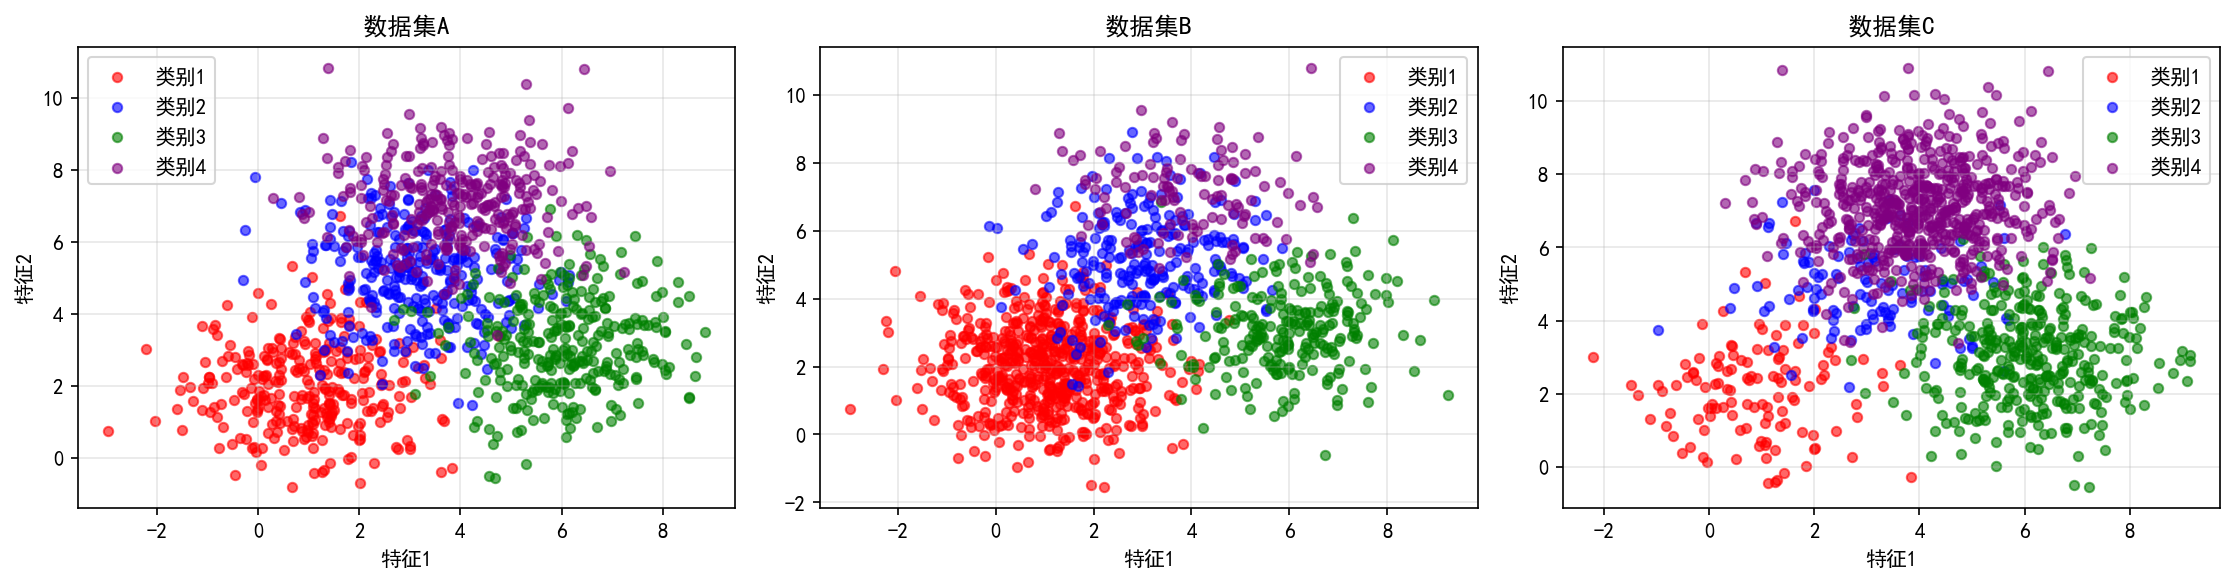
\includegraphics[width=0.95\textwidth]{1.png}
\caption{三个数据集的样本分布散点图。(从左到右分别为数据集A(均衡先验)、B(偏斜先验1)、C(偏斜先验2)。红色、蓝色、绿色、紫色点分别代表类别1-4。可以观察到四个类别的中心位置与设定的均值向量一致,且由于协方差矩阵相同,各类别的分布形状相似但中心位置不同,存在一定的重叠区域。(仅供解释,报告里不必要有,后续图同样)}
\label{fig:dataset_dist}
\end{figure}

\subsection{参数估计分类器性能分析}

\begin{table}[htbp]
\centering
\caption{参数估计方法在不同数据集上的分类准确率}
\begin{tabular}{ccccccc}
\toprule
数据集 & 分类规则 & 总体准确率 & 类别1准确率 & 类别2准确率 & 类别3准确率 & 类别4准确率 \\
\midrule
\multirow{2}{*}{A} & 似然率测试 & 0 & 0 & 0 & 0 & 0 \\
& MAP规则 & 0 & 0 & 0 & 0 & 0 \\
\midrule
\multirow{2}{*}{B} & 似然率测试 & 0 & 0 & 0 & 0 & 0 \\
& MAP规则 & 0 & 0 & 0 & 0 & 0 \\
\midrule
\multirow{2}{*}{C} & 似然率测试 & 0 & 0 & 0 & 0 & 0 \\
& MAP规则 & 0 & 0 & 0 & 0 & 0 \\
\bottomrule
\end{tabular}
\end{table}


\begin{figure}[htbp]
\centering
\includegraphics[width=0.95\textwidth]{confusion_matrices.png}
\caption{三个数据集在不同分类规则下的混淆矩阵热图。行表示真实类别,列表示预测类别。对角线元素表示正确分类的样本数。(这一块可以做适当的分析,如:在数据集B和C中,MAP规则相比似然率测试规则在多数类别(B中的类别1和C中的类别4)上表现更好,但在少数类别上准确率有所下降,体现了先验概率对分类决策的影响。)}
\label{fig:confusion_matrix}
\end{figure}

\subsection{核密度估计参数优化分析}

\begin{table}[htbp]
\centering
\caption{不同数据集下的最优带宽参数及对应准确率}
\begin{tabular}{ccccc}
\toprule
数据集 & 分类规则 & 最优$h$值 & 交叉验证准确率 & 测试集准确率 \\
\midrule
A & 似然率测试 & 0 & 0 & 0 \\
A & MAP规则 & 0 & 0 & 0 \\
B & 似然率测试 & 0 & 0 & 0 \\
B & MAP规则 & 0 & 0 & 0 \\
C & 似然率测试 & 0 & 0 & 0 \\
C & MAP规则 & 0 & 0 & 0 \\
\bottomrule
\end{tabular}
\end{table}

\begin{figure}[htbp]
\centering
\includegraphics[width=0.95\textwidth]{bandwidth_analysis.png}
\caption{带宽参数$h$对分类准确率的影响分析}
\label{fig:bandwidth_analysis}
\end{figure}

\begin{figure}[htbp]
\centering
\includegraphics[width=0.95\textwidth]{kernel_density_estimation.png}
\caption{核密度估计可视化结果。(每行对应一个数据集,左列为密度等高线图(以类别0为例),右列为分类结果图(正确分类用圆圈表示,错误分类用叉号表示)。等高线可以用contour()函数画)}
\label{fig:kernel_density}
\end{figure}

\subsection{k-近邻密度估计性能分析}

\begin{table}[htbp]
\centering
\caption{k-近邻方法中不同k值的分类准确率比较}
\begin{tabular}{ccccccc}
\toprule
数据集 & 分类规则 & k=1 & k=3 & k=5 & k=8 & k=10 \\
\midrule
\multirow{2}{*}{A} & 似然率测试 & 0 & 0 & 0 & 0 & 0 \\
& MAP规则 & 0 & 0 & 0 & 0 & 0 \\
\midrule
\multirow{2}{*}{B} & 似然率测试 & 0 & 0 & 0 & 0 & 0 \\
& MAP规则 & 0 & 0 & 0 & 0 & 0 \\
\midrule
\multirow{2}{*}{C} & 似然率测试 & 0 & 0 & 0 & 0 & 0 \\
& MAP规则 & 0 & 0 & 0 & 0 & 0 \\
\bottomrule
\end{tabular}
\end{table}

\begin{figure}[htbp]
\centering
\includegraphics[width=0.95\textwidth]{knn_analysis.png}
\caption{k值对k-近邻分类准确率的影响}
\label{fig:knn_analysis}
\end{figure}



\subsection{方法综合性能比较}

\begin{table}[htbp]
\centering
\caption{三种估计方法在三个数据集上的最优性能比较}
\begin{tabular}{cccccc}
\toprule
数据集 & 估计方法 & 分类规则 & 最优参数 & 准确率 & 相对性能 \\
\midrule
\multirow{6}{*}{A} & \multirow{2}{*}{参数估计} & 似然率测试 & - & 0 & \multirow{2}{*}{基准} \\
& & MAP规则 & - & 0 & \\
\cmidrule{2-6}
& \multirow{2}{*}{核密度} & 似然率测试 & $h=0$ & 0 & 0\% \\
& & MAP规则 & $h=0$ & 0 & 0\% \\
\cmidrule{2-6}
& \multirow{2}{*}{k-近邻} & 似然率测试 & $k=0$ & 0 & 0\% \\
& & MAP规则 & $k=0$ & 0 & 0\% \\
\midrule
\multirow{6}{*}{B} & \multirow{2}{*}{参数估计} & 似然率测试 & - & 0 & 基准 \\
& & MAP规则 & - & 0 & 0\% \\
\cmidrule{2-6}
& \multirow{2}{*}{核密度} & 似然率测试 & $h=0$ & 0 & 0\% \\
& & MAP规则 & $h=0$ & 0 & 0\% \\
\cmidrule{2-6}
& \multirow{2}{*}{k-近邻} & 似然率测试 & $k=0$ & 0 & 0\% \\
& & MAP规则 & $k=0$ & 0 & 0\% \\
\midrule
\multirow{6}{*}{C} & \multirow{2}{*}{参数估计} & 似然率测试 & - & 0 & 基准 \\
& & MAP规则 & - & 0 & 0\% \\
\cmidrule{2-6}
& \multirow{2}{*}{核密度} & 似然率测试 & $h=0$ & 0 & 0\% \\
& & MAP规则 & $h=0$ & 0 & 0\% \\
\cmidrule{2-6}
& \multirow{2}{*}{k-近邻} & 似然率测试 & $k=0$ & 0 & 0\% \\
& & MAP规则 & $k=0$ & 0 & 0\% \\
\bottomrule
\end{tabular}
\end{table}

\begin{figure}[htbp]
\centering
\includegraphics[width=0.95\textwidth]{final_comparison.png}
\caption{三种估计方法在三个数据集上的最终性能对比。每个子图对应一个数据集,横轴为不同的估计方法和分类规则组合,纵轴为分类准确率。}
\label{fig:final_comparison}
\end{figure}

\section{实验总结与讨论}

\subsection{主要发现}
\begin{enumerate}
    \item \textbf{先验概率的显著影响}:。
    
    \item \textbf{参数方法 vs 非参数方法}:
    \begin{itemize}
        \item \textbf{参数方法}:
        \item \textbf{非参数方法}:
    \end{itemize}
    
    
    \item \textbf{参数选择的敏感性}:
    \begin{itemize}
        \item 核密度估计中,
        \item k-近邻方法中,
    \end{itemize}
\end{enumerate}

\subsection{方法优缺点讨论}

\textbf{参数估计方法:}
\begin{itemize}
    \item \textbf{优点}:
    \item \textbf{缺点}:
\end{itemize}

\textbf{核密度估计方法:}
\begin{itemize}
    \item \textbf{优点}:
    \item \textbf{缺点}:
\end{itemize}

\textbf{k-近邻密度估计:}
\begin{itemize}
    \item \textbf{优点}:
    \item \textbf{缺点}:
\end{itemize}

\subsection{心得体会}
\end{document}
